\chapter{Radioactive Decay}
\section{Radioactivity}
Many nuclides present in the universe are unstable and spondaneously change in to other nuclides by a process pulled radioactive decay. The phenomina is known as radioactivity and was discovered Antonine Bequerel. Following three aspects of radioactivity are extraordinary from the perspective of classical physics.\\
(i) \quad When a nucleus undergo $\alpha$ or $\beta$ decays its atomic number $Z$ changes and it becomes the nucleus of a different form. Obviously the elements are not immutable. (not transformed to the original one naturally)\\
(ii)\quad The energy liberated during radioactive decay comes from with in the individual nuclei without external excitation.\\
(iii)\quad Radioactive decay is statistical process.
\subsection{Radioactive Decay}
There are five different ways in which a radio action nuclide can decay . That are by emitting an alpha ($ ^4_2He$ nuclei), beta(electrons),gamma(high energy photons) particles or by positron emission  and electron capture. In which alpha particle is +vely charged and $P$ particles are -vely charged and the gamma rays are natural. The penitrating power is maximum for  gamma rays. The penitrating power of $\alpha$,$\beta$,$\gamma$, particle can be picturized as\\
\begin{figure}[H]
	\centering
	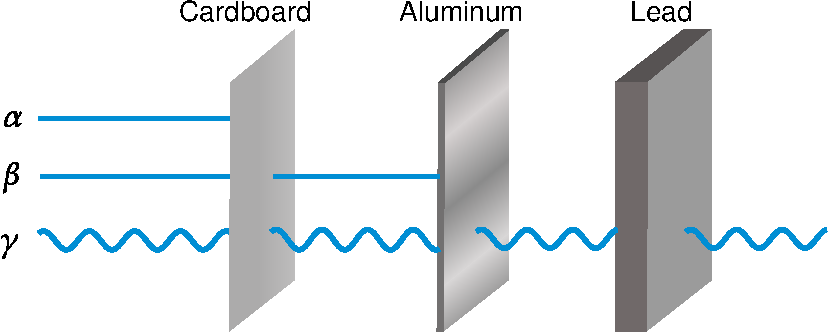
\includegraphics[height=3cm,width=8cm]{diagram-20220307(6)-crop}
	\caption{}
	\label{}
\end{figure}
Radioactive Decay\\
	\begin{table}[H]
	\centering
	\renewcommand*{\arraystretch}{1.5}
	\begin{tabular}{|p{2.5cm} |p{3.5cm}|p{4cm}|p{3.7cm} |}
	\hline Decay &Reason for instability& Transformation & Example \\
	\hline Alpha decay &Nucleus is too large.& ${ }_{2}^{A} X \rightarrow{ }_{Z-2}^{A-4} Y+{ }_{2}^{4} \mathrm{He}$ & ${ }_{29}^{238} \mathrm{U} \rightarrow{ }_{90}^{234} \mathrm{Th}+{ }_{2}^{4} \mathrm{He}$ \\
	 & &Emission of $\alpha$-particle reduces size of nucleus.& \\
	\hline
	Beta decay &Nucleus has too many neutrons relative to number of protons.& ${ }_{2}^{A} X \rightarrow{ }_{Z+1}^{A} Y+e^{-}$ & ${ }_{6}^{14} \mathrm{C} \rightarrow{ }_{7}^{14} \mathrm{~N}+e^{-}$ \\
	 & &Emission of electron by neutron in nucleus changes the neutron to a proton.& \\
		\hline
	Gamma decay &Nucleus has excess energy.& ${ }_{Z}^{A} X^{*} \rightarrow{ }_{Z}^{A} X+\gamma$ & ${ }_{87}^{87} \mathrm{Cu}+{ }_{38}^{8} \mathrm{Sr}^{*} \rightarrow{ }_{38}^{87} \mathrm{Sr}+\gamma$ \\
	 & &Emission of $\gamma$-ray reduces energy of the nucleus.& \\
		\hline
	Electron capture &Nucleus has too many protons relative to number of neutrons.& ${ }_{Z}^{A} X+e^{-} \rightarrow_{z-1}^{A} Y$ & ${ }_{64}^{A} \mathrm{Cu}+e^{-} \rightarrow{ }_{28}^{64} \mathrm{Ni}$ \\
	 & &Capture of electron by protons changes the proton to a neutron.& \\
		\hline
	Positron emission &Nucleus has too many protons relative to number of neutrons.& ${ }_{2}^{A} X \rightarrow{ }_{-1}^{A} Y+e^{+}$ & ${ }_{29}^{64} \mathrm{Cu} \rightarrow{ }_{28}^{64} \mathrm{Ni}+e^{+}$ \\
	 & &Emission of positron by proton in nucleus changes the proton to a neutron.& \\
	\hline
	\end{tabular}
\end{table}





${ }^{+}$The * denotes an excited nuclear state and $\gamma$ denotes a gamma-ray photon.
\subsection{Activity}
The activity of a sample of any radioactive nuclide is the rate at which the nuclei of its constituent atoms decay.If $N$ is the number of nuclei present in the sample at a certain time, its activity $R$ is given by
\begin{align*}
R&=\frac{-dN}{dt}
\intertext{The minus sign is used to make $R$ a positive quantity since $\frac{dN}{dt}$ is negative. The time variation of activity is followed by the formula, }
R&=R_0e^{-\lambda t}
\end{align*}
Where $\lambda$ is called decay constant or disintegration constant.
\subsection{Radioactive Decay Law}
(i) \quad On emission of $\alpha$ or $\beta$ particle which is usually but not invariably accompanied by $\gamma$-ray emission, the emitting parent nuclide transforms in to a new daughter element. The daughter element again is radioactive. So that the process of successive disintegration continues till the original active parent nuclid get transformed in to a stable one.\\
(2)\quad The rate of radioactive disintegration that is the number of atoms that break up at any instant of time $t$ is directly preportional to the number $N$ of active nuclides present in the sample at that instant.\\
In other words "The probability per unit time that a nucleus will decay is a constant and is independent of time". $\lambda$ is the probability per unit time. Which is a constant \\
\subsubsection{Decay Equation}
The mathematical representation of the law of radioactive decay is 
\begin{align}
&-\frac{d N}{d t} \alpha N\\
\frac{d N}{d t}&=\lambda N, \lambda \text{decay constant}\\
\frac{d N}{N}&=-\lambda d t\\
\int \frac{d N}{N}&=-\lambda \int d t\\
\ln N&=-\lambda t+A\\
\text{A is the constant}&\text{ of integration.}\\
\text{at $t=0 \quad N=N_{0}$}&\text{ the initial number of unclides.}\\
A&=\ln N_{0}\\
\therefore \ln N&=-\lambda t+\ln N _0\\
\ln \frac{N }{ N_{0}}&=-\lambda t\\
\frac{N}{N_0}&=e^{-\lambda t}\\
\text{$\mathrm{N}=\mathrm{N}_{0} \mathrm{e}^{-\lambda \mathrm{t}}$ which is the }&\text{  equation form of the law of radioactive decay}\\
\text{we know,}\quad\\
-\frac{d N}{d t}&=R \label{nuclear decay eq}\\
\text{and }-\frac{d N}{d t}&=\lambda N\label{nuclear decay eq 2}\\
\text{So.} R&=\lambda N
\end{align}
\subsection{Half Life ($T_\frac{1}{2}$)}
\begin{align*}
\text{Half life is the time }&\text{($t=T_\frac{1}{2}$) at which the activity $R$ drops to $\frac{1}{2}R_0$}\\
R&=R_{0} e^{-\lambda t}\\
\frac{1}{2} R_{0}&=R _0 e^{-\lambda T_\frac{1}{2}}\\
e^\lambda T_\frac{1}{2}&=2\\
\lambda T_\frac{1}{2}&=\ln 2=.693\\
T_\frac{1}{2}&=\frac{\ln 2}{\lambda}=\frac{0.693}{\lambda}\\
\text{From half-life the decay constant}&\text{ $\gamma$ of a radioactive nuclei can be found out }\\
\lambda&=\frac{-693}{T_\frac{1}{2}}\\
\text{The decay constant of }&\text{radionuclide whose half life is $5 h$ is}\\
\lambda=\frac{0.693}{T _\frac{1}{2}}&=\frac{0.693}{5 \times 3600 \mathrm{~S}}=3.85 \times 10^{-5} 8^{-1}\\
\text{The larger the decay constant, the}&\text{ greater the chance the given nucleus will decay in a certain period of time}
\end{align*}
\subsection{Mean Lifetimer $\left\langle \bar{T}\right\rangle $ or Average Life }
\begin{align*}
\text{The mean life time of a nuclide }&\text{is the resiprocal of its decay probability per unit time.}\\
\bar{T}&=\frac{1}{\lambda}\\
\text{Hence}
\bar{T}&=\frac{T_\frac{1}{2}}{0.693}=1.44 T_\frac{1}{2}\\
\text{$\bar{T}$ is nearly half }&\text{again more than $T_{\frac{1}{2}}\left[\left(1+\frac{1}{2}\right) T_\frac{1}{2}\right]$}\\
\text{The mean life time of a }&\text{radionuclide whose half life is $5 hr$ is}\\
\bar{T}&=1.44 \ T_{\frac{1}{2}}=1.44 \times 5=7.2 hr
\end{align*}
\subsection{Units of Radioactivity}
\begin{enumerate}
	\item \textbf{ Curie (Ci)}
	\begin{align*}
	\intertext{The traditional units of activity is curie (Ci). Which can be defined as the activity of $1g$ of radium. $1g$ radius have $3\cdot7 \times 10^{10}$ disintegration per second . so}
	\text{$1 $  Curie (Ci) $=3\cdot7\times10^6$ disintegration/sec}\\
	\text{$\therefore$ \quad the activity of $1gm$ of radium is equal to curie.}\\
	\text{$1m \ Ci=10^{-3} Ci=3\cdot 7 \times 10^7 $ disintegration/sec}\\
	\text{$1m \ Ci=10^{-6} Ci=3\cdot 7 \times 10^4 $ disintegration/sec}
	\end{align*}
	\item \textbf{Rutherford (rd)}
	\begin{align*}
	1 \text{ Rutherford } (rd) &= 10^6 \text{ disintegration/sec}\\
	1 m\  rd&=10^{-3}\  rd\\
	1 m\  rd&=10^{-6}\  rd
	\end{align*}
	\item \textbf{Bequerel (Bq)}
	\begin{align*}
	\text{Bequerel is the $SI$ }&\text{unit of radioactivity}\\
	1 Bq&=1 \text{ disintegration/sec}\\
	1Ci&=3\cdot7\times10^{10}Bq =37GB_q=37\times10^9Bq\\
	MB_q&=10^6Bq\\
	GB_q&=10^9Bq
	\end{align*}
\end{enumerate}
\section{Successive Growth}
Consider $A,B$ and $C$ are the first three members of a radioactive series. $C$ is a stable nuclei.\\
$\begin{array}{llll}  
&A\quad \longrightarrow & B\quad  \longrightarrow C  \\ 
t=0 & N_0 & O & O  \\ 
t=t & N_1 & N_2 & N_3\end{array}$